\pdfsuppresswarningpagegroup=1

\PassOptionsToPackage{dvipsnames}{xcolor}

\documentclass[
    aspectratio=169,
    %handout,
]{beamer}

\usetheme{Boadilla}
\usecolortheme{seahorse}
\usepackage{pifont}
\usepackage{pgfplots}
\usepackage{svg}
\usepackage{t1enc}
\usepackage{bbding}
\usepackage{enumitem}
\usepackage{fontawesome5}
\usepackage{minted}
\usepackage[hungarian]{babel}
\usepackage[none]{hyphenat}
\usepackage[absolute,overlay]{textpos}
\usepackage{qrcode}
\usepackage{amsfonts}

\pgfplotsset{
    tick label style = {font = {\fontsize{8 pt}{14 pt}\selectfont}},
    every axis label = {font = {\fontsize{8 pt}{14 pt}\selectfont}},
    label style = {font = {\fontsize{10 pt}{20pt}\selectfont}},
    legend style = {font = {\fontsize{6 pt}{10 pt}\selectfont}},
}

\setenumerate{
    label=\arabic*.,
    itemsep=3pt,
    topsep=3pt,
}
  
\setitemize{
    label=\usebeamerfont*{itemize item}%
    \usebeamercolor[fg]{itemize item}
    \usebeamertemplate{itemize item}
}
  
\newlist{logolist}{itemize}{1}
\setlist[logolist,1]{
    label={},
    leftmargin=4em
}

\titlegraphic{
\includegraphics[width=2cm]{elte_cimer_szines}}
\title[HoloDB]{HoloDB: Relációs demóadatok konzisztens on-the-fly generálása\\ deklaratív konfigurációból}
\author[Horváth Dávid]{Horváth Dávid \\ ~ \\ { \footnotesize Témavezető: dr. Vincellér Zoltán, mesteroktató }}
\institute[ELTE-IK]{ELTE Informatikai Kar, Információs Rendszerek Tanszék}
\date{2025}

\newcommand{\slidetitle}[2]{\frametitle{{\small #1 ~ \ding{226} ~ } \normalsize \textbf{#2} }}

\newcommand{\greencheck}{{\color{green!65!black}\ding{51}}}

\newcommand{\textbftt}[1]{{\fontfamily{lmtt}\fontseries{b}\selectfont{#1}}}

\newcommand{\brqr}{
    \begin{textblock*}{2cm}[0,0](\dimexpr\paperwidth-2.5cm\relax,\dimexpr\paperheight-2.5cm\relax)
        \resizebox{2cm}{!}{\qrcode{https://github.com/miniconnect/holodb}}
    \end{textblock*}
}

\newcommand{\best}[1]{{\color{green}\underline{#1}}}

\newcommand{\bad}[1]{{\color{red}#1}}

\begin{document}
\beamertemplatenavigationsymbolsempty

\begin{frame}[plain,noframenumbering]
    \titlepage
\end{frame}

\begin{frame}
    \frametitle{Tartalom}
    \hfill
    \parbox[t]{.95\textwidth}{
        \begin{minipage}[c][0.6\textheight]{\textwidth}
        \tableofcontents
        \end{minipage}
    }
\end{frame}

\section{A probléma: adatbázist akarok, most!}
\def\sectionshorttitle{\arabic{section}. A probléma}

\begin{frame}[fragile]
    \slidetitle{\sectionshorttitle}{Adatbázist akarok, most!}
    
    \begin{minipage}[c]{0.63\textwidth}
        \begin{logolist}
            \setlength\itemsep{1.2em}
            \item[\raisebox{-0.75em}{
\includegraphics[width=2em,height=2em]{image/dbnow-mock}}]
                \begin{minipage}[c]{\linewidth}~~\textbf{mockolás, fejlesztés} \par ~~~~
                    csak legyen ott valami, hogy fusson
                \end{minipage}
            \item[\raisebox{-0.75em}{
\includegraphics[width=2em,height=2em]{image/dbnow-prot}}]
                \begin{minipage}[c]{\linewidth}~~\textbf{tervezés, prototipizálás, kísérletezés} \par ~~~~
                    szeretnénk folyamatosan újragondolni
                \end{minipage}
            \item[\raisebox{-0.75em}{
\includegraphics[width=2em,height=2em]{image/dbnow-test}}]
                \begin{minipage}[c]{\linewidth}~~\textbf{integrált tesztelés} \par ~~~~
                    kellenének adatok a tesztfuttatáshoz
                \end{minipage}
            \item[\raisebox{-0.75em}{
\includegraphics[width=2em,height=2em]{image/dbnow-pres}}]
                \begin{minipage}[c]{\linewidth}~~\textbf{bemutatók, koncepciótervek} \par ~~~~
                    értelmes adathalmaz a demózáshoz
                \end{minipage}
            \item[\raisebox{-0.75em}{
\includegraphics[width=2em,height=2em]{image/dbnow-stud}}]
                \begin{minipage}[c]{\linewidth}~~\textbf{oktatás} \par ~~~~
                    egységes homokozó adatbázis tanulóknak
                \end{minipage}
        \end{logolist}
        \pause
    \end{minipage}%
    \hspace*{\fill}%
    \begin{minipage}[c]{0.35\textwidth}
        \centering
        
        \includegraphics[width=\textwidth]{diagram/database-tasks-compressed}
    \end{minipage}%
    \hspace*{\fill}%
\end{frame}

\begin{frame}[fragile]
    \slidetitle{\sectionshorttitle}{A szokásos megközelítések}
    
    \begin{minipage}[c]{0.58\textwidth}
        \begin{logolist}
            \setlength\itemsep{2em}
            \Large
            \item[\raisebox{-0.4em}{\includesvg[width=1.25em]{image/solution-copy}}]
                    ~produkciós adatbázis másolása
            \item[\raisebox{-0.4em}{\includesvg[width=1.25em]{image/solution-anonymize}}]
                    ~anonimizálás
            \item[\raisebox{-0.4em}{\includesvg[width=1.25em]{image/solution-generate}}]
                    ~adatgenerálás
            \item[\raisebox{-0.4em}{\includesvg[width=1.25em]{image/solution-mock}}]
                    ~lekérdezések ad hoc mockolása
        \end{logolist}
        \pause
    \end{minipage}%
    \hspace*{\fill}%
    \begin{minipage}[c]{0.35\textwidth}
        \centering
        
        \begin{minipage}[t]{0.48\textwidth}
            \centering
            
            
\includegraphics[width=0.45\textwidth, frame]{image/mostly-ai}\par
            \textbf{MOSTLY AI}
            
            \vspace{5pt}
            
            
\includegraphics[width=0.45\textwidth, frame]{image/tonic}\par
            \textbf{Tonic}
        \end{minipage}%
        \hspace*{\fill}%
        \begin{minipage}[t]{0.48\textwidth}
            \centering
            
            
\includegraphics[width=0.45\textwidth, frame]{image/genrocket}\par
            \textbf{GenRocket}
            
            \vspace{5pt}
            
            
\includegraphics[width=0.45\textwidth, frame]{image/delphix}\par
            \textbf{Delphix}
        \end{minipage}%
        \hspace*{\fill}%
        
        \pause
        
        \vspace{10pt}
        
        
\includegraphics[width=0.47\textwidth, frame]{image/faker}\par
        \textbf{Faker}
        
    \end{minipage}%
    \hspace*{\fill}%
\end{frame}

\begin{frame}
    \slidetitle{\sectionshorttitle}{Alternatív ihletforrás}
    
    \centering
    
    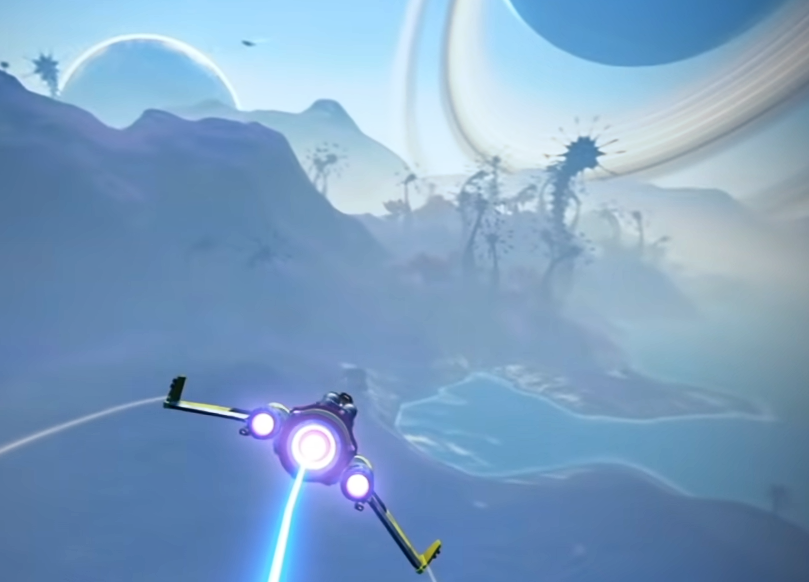
\includegraphics[height=0.8\textheight]{image/nomanssky}
    
    \smallskip
    
    \footnotesize{Részlet a \textit{No Man's Sky Origins} játékból (hivatalos trailer)}
\end{frame}

\section{A HoloDB felépítése}
\def\sectionshorttitle{\arabic{section}. Felépítés}

\begin{frame}
    \slidetitle{\sectionshorttitle}{Elvárások egy új megoldással szemben}
    
    \begin{itemize}
        \setlength\itemsep{0.5em}
        \item {\color{red}relációs adatmodell}re épül
        \item {\color{red}deklaratív}, finomhangolható, könnyen bővíthető
        \item {\color{red}nincs preparálás}i folyamat, szinte azonnal elindul
        \item óriás adatmennyiséget is képes szimulálni, szinte {\color{red}tárhelyigény nélkül}
        \item az adatokat csak elérésükkor, on-the-fly számítja
        \item indexelt, a runtime teljesítmény elfogadható
        \item determinisztikus, {\color{red}koherens}, skálázható
        \item opcionálisan írható
    \end{itemize}
\end{frame}

\begin{frame}[fragile]
    \slidetitle{\sectionshorttitle}{Konfiguráció-példa}
    
    \centering
    
    \begin{minipage}[c]{0.47\textwidth}
        \centering
        
        \begin{minted}[
            fontsize=\tiny,
            framesep=4pt,
            frame=single,
            framerule=1.5pt,
            rulecolor=\color{gray!30}
        ]{yaml}
seed: 425364
schemas:
  - name: shop
    tables:
      - name: customers
        size: 5
        columns:
          - name: id
            mode: COUNTER
          - name: firstname
            valuesBundle: forenames
          - name: lastname
            valuesBundle: surnames
          - name: birth
            valuesRange: [1950, 2000]
      - name: orders
        size: 12
        columns:
          - name: id
            mode: COUNTER
          - name: cid
            valuesForeignColumn: [customers, id]
          - name: product
            valuesBundle: fruits
          - name: quantity
            valuesRange: [1, 10]
        \end{minted}
        
        {\footnotesize\texttt{config.yaml}} \pause
    \end{minipage}%
    \hspace*{\fill}
    \begin{minipage}[c]{0.35cm}
        {\Large $\Rightarrow$}
    \end{minipage}%
    \hspace*{\fill}
    \begin{minipage}[c]{0.45\textwidth}
        
        \centering
        
        \normalsize \texttt{customers}
        \vspace{0.1cm}
        
        \tiny
        \begin{tabular}{ |r|l|l|r| }
        \hline
           id & firstname & lastname & birth \\
        \hline
            1 & Howard & Anderson & 1968 \\
            2 & Rebecca & Ferguson & 1959 \\
            3 & Jeremy & Moore & 2000 \\
            4 & Julie & Ellis & 1951 \\
            5 & Kathleen & Cook & 1971 \\
        \hline
        \end{tabular}
        
        \vspace{0.5cm}
        
        \normalsize \texttt{orders}
        \vspace{0.1cm}
        
        \tiny
        \begin{tabular}{ |r|r|l|r| }
        \hline
            id & cid & ~~product & quantity \\
        \hline
            1 & 5 & date & 10 \\
            2 & 2 & orange & 1 \\
            3 & 2 & sloe & 2 \\
            4 & 3 & melon & 7 \\
            5 & 5 & guava & 9 \\
            6 & 3 & orange & 6 \\
            7 & 2 & plantain & 3 \\
            8 & 4 & pear & 7 \\
            9 & 4 & papaya & 9 \\
            10 & 5 & lime & 9 \\
            11 & 3 & sloe & 4 \\
            12 & 1 & strawberry & 1 \\
        \hline
        \end{tabular}
    \end{minipage}
\end{frame}

\begin{frame}
    \slidetitle{\sectionshorttitle}{Az arhitektúra áttekintése}
    
    \centering
    
    \begin{minipage}[c]{0.4\textwidth}
        \begin{overprint}
            \onslide<1>\centerline{\includegraphics[width=\textwidth]{diagram/simplearch-0}}
            \onslide<2-3>\centerline{\includegraphics[width=\textwidth]{diagram/simplearch-1}}
        \end{overprint}
    \end{minipage}%
    \hspace*{\fill}
    \begin{minipage}[c]{0.29\textwidth}
        \begin{overprint}
            \onslide<2-3>\begin{itemize}
                \item \texttt{Schema}
                \item \texttt{Table}
                \item \texttt{Column}
                \item \texttt{ColumnDefinition}
                \item {\only<3>{\color{beamer@blendedblue}\underline}{\texttt{Source}}}
                \item \texttt{Row}
                \item \texttt{TableIndex}
                \item \texttt{FulltextIndex}
                \item \texttt{SpatialIndex}
                \item \texttt{TableSelection}
            \end{itemize}
        \end{overprint}
    \end{minipage}%
    \begin{minipage}[c]{0.29\textwidth}
        \begin{overprint}
            \onslide<3>\centerline{\includegraphics[width=\textwidth]{diagram/storage-source}}
        \end{overprint}
    \end{minipage}%
    \hspace*{\fill}%
\end{frame}

\begin{frame}
    \slidetitle{\sectionshorttitle}{Alapvető adattípus: LargeInteger}
    
    \begin{minipage}[t]{0.6\textwidth}
        \centering
        
        \vspace{0.5em}
        
        \begin{itemize}
            \setlength\itemsep{0.5em}
            \item kis és óriás egészekkel is működik
            \item a konverzió automatikus és egyértelmű
            \item kis számokon gyors (\texttt{long} aritmetika)
            \item memóriaigénye minimális
            \item duplikálja a \texttt{BigInteger} metódusait
            \item további hasznos metódusokkal bővíti
            \item nincsenek függőségei
        \end{itemize}
    \end{minipage}%
    \begin{minipage}[t]{0.4\textwidth}
        \centering
        
        \vspace{0.05em}
        
        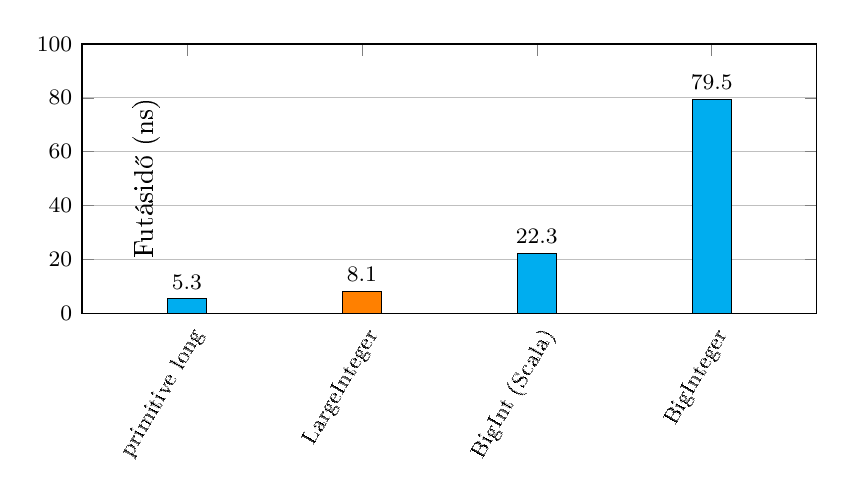
\begin{tikzpicture}[font=\footnotesize]
            \begin{axis}[
                    symbolic x coords={primitive long,,LargeInteger,,BigInt (Scala),,BigInteger},
                    xticklabel style={rotate=60,anchor=north east},
                    xtick={primitive long,LargeInteger,BigInt (Scala),BigInteger},
                    ylabel={Futásidő (ns)},
                    y label style={at={(0.12,0.5)}},
                    width={0.9\textwidth},
                    height=5cm,
                    ymajorgrids,
                    ymin=0,
                    ymax=100,
                    bar width=0.5cm,
                    enlarge x limits=0.2,
                    nodes near coords,
                    nodes near coords align={vertical},
                ]
                \addplot[ybar,fill=cyan] coordinates { (primitive long,5.3) };
                \addplot[ybar,fill=orange] coordinates { (LargeInteger,8.1) };
                \addplot[ybar,fill=cyan] coordinates { (BigInt (Scala),22.3) };
                \addplot[ybar,fill=cyan] coordinates { (BigInteger,79.5) };
            \end{axis}
        \end{tikzpicture}
    \end{minipage}
    
    \begin{flushright}
        { \footnotesize Benchmark: kis számokon végzett sokféle művelet ~~~~~ }
    \end{flushright}
\end{frame}

\begin{frame}
    \slidetitle{\sectionshorttitle}{Alapvető adattípus: TreeRandom}
    
    \begin{minipage}[c]{0.5\textwidth}
        \vspace{0.5em}
        
        {\color{beamer@blendedblue}Hierarchikus véletlengenerátor}
        
        \vspace{0.2cm}
        
        \begin{itemize}
            \item kulcs megadásával alpéldány
            \item egyenlő kulcs: egyenlő alpéldány
            \item egyenlő példány: egyező kimenet
        \end{itemize}

        \vspace{0.7cm}
        
        {\color{beamer@blendedblue}Gyenge követelmények}

        \vspace{0.2cm}
        
        \begin{itemize}
            \item véletlenszerű kimenetet ad
            \item eltérő példány: eltérő kimenet
        \end{itemize}

        \begin{overprint}
            \onslide<6>\begin{flushright}
                \vspace{2.5em}
                
                { \tiny \color{BrickRed}
                    \texttt{871121}{\color{RoyalPurple},}%
                    \texttt{"schema1"}{\color{RoyalPurple},}%
                    \texttt{"table1"}{\color{RoyalPurple},}%
                    \texttt{"description"}{\color{RoyalPurple},}%
                    \texttt{3}{\color{RoyalPurple},}%
                    \texttt{"text"} {\color{RoyalPurple}$\rightarrow$}
                    seed
                }
            \end{flushright}
        \end{overprint}
    \end{minipage}%
    \begin{minipage}[c]{0.5\textwidth}
        \begin{overprint}
            \onslide<2>\centerline{\includegraphics[height=0.85\textheight]{diagram/treerandom-0}}
            \onslide<3>\centerline{\includegraphics[height=0.85\textheight]{diagram/treerandom-1}}
            \onslide<4>\centerline{\includegraphics[height=0.85\textheight]{diagram/treerandom}}
            \onslide<5-6>\centerline{\includegraphics[height=0.85\textheight]{diagram/treerandom-nonindexed}}
            \onslide<7>\centerline{\includegraphics[height=0.85\textheight]{diagram/treerandom-indexed}}
        \end{overprint}
    \end{minipage}
\end{frame}

\begin{frame}[t,fragile]
    \slidetitle{\sectionshorttitle}{Alapvető adattípus: Permutation}
    
    \vspace{0.5em}
    
    \begin{minipage}[t]{0.37\textwidth}
        \vspace{0.2em}
        
        {\color{beamer@blendedblue}Követelmények permutációkra:}

        \vspace{0.2cm}
        
        \begin{itemize}
            \item $\mathbb{N} \to \mathbb{N}$
            \item tetszőleges méretű
            \item hatékony inverz
            \item véletlenszerűség látszata
            \item SIT
            \item AMET
        \end{itemize}
    \end{minipage}%
    \begin{minipage}[t]{0.6\textwidth}
        \centering
        
        {\footnotesize
        \begin{tabular}[t]{|l||r|r|r|r|} 
        \hline
        ~
            & \begin{tabular}{c} \textbftt{mem} \\ {\footnotesize{(bytes)}} \end{tabular}
            & \begin{tabular}{c} \textbftt{paq8/4} \\ {\footnotesize{(\%)}} \end{tabular}
            & \begin{tabular}{c} \textbftt{create} \\ {\footnotesize{(ns)}} \end{tabular}
            & \begin{tabular}{c} \textbftt{at×30} \\ {\footnotesize{(ns)}} \end{tabular}\\
        \hline\hline
        \textbftt{FAV} & 648 & 31,54 & 968 &  2~040 \\
        \hline
        \textbftt{MP1} & \best{152} & \bad{0,19} & \best{267} & \best{161} \\
        \hline
        \textbftt{FEI-F-4} & 608 & 19,56 & 660 & 8~800 \\
        \hline
        \textbftt{FEI-S-2} & \bad{212~312} & 97,08 & 434 & \bad{32~221} \\
        \hline
        \textbftt{FPE1} & \bad{211~352} & \best{97,07} & 540 & \bad{67~155} \\
        \hline
        \end{tabular}
        }
        
        \vspace{1.5em}
        
        \begin{minipage}[b]{0.25\textwidth}
            \centering
            
\includegraphics[width=0.95\textwidth]{image/permutation-fav.png}
            \par FAV
        \end{minipage}%
        \begin{minipage}[b]{0.25\textwidth}
            \centering
            
\includegraphics[width=0.95\textwidth]{image/permutation-mp1.png}
             \par MP1
        \end{minipage}%
        \begin{minipage}[b]{0.25\textwidth}
            \centering
            
\includegraphics[width=0.95\textwidth]{image/permutation-feif4.png}
            \par FEI-F-4
        \end{minipage}%
        \begin{minipage}[b]{0.25\textwidth}
            \centering
            
\includegraphics[width=0.95\textwidth]{image/permutation-feis2.png}
            \par FEI-S-2
        \end{minipage}%
        
    \end{minipage}
    
\end{frame}

\begin{frame}
    \slidetitle{\sectionshorttitle}{Általános kétlépéses értékkiosztás}
    
    \centering
    
    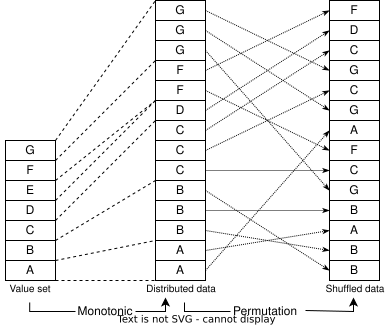
\includegraphics[height=0.7\textheight]{diagram/distribution}
    
    A kétlépéses értékkiosztás alapelve: \par
    visszafejthető disztribúció és permutáció kompozíciója
\end{frame}

\begin{frame}
    \slidetitle{\sectionshorttitle}{Írhatósági réteg}
    
    \begin{minipage}[c]{0.65\textwidth}
        {\color{beamer@blendedblue}A \texttt{DiffTable} dekorátor}
        
        \begin{itemize}
            \item csak olvassa az alárendelt táblaobjektumot
            \item amíg nincs módosítás, átlátszóan működik
            \item memóriában tárolja a módosításokat
            \item átírhatja a lekérést és összefésülheti az eredménytáblát
        \end{itemize}
        
        \vspace{0.4cm}
        
        {\color{beamer@blendedblue}Tranzakciókezelés}
        
        \begin{itemize}
            \item kétféle tranzakciós stratégia: írási ablakok vagy MVCC
            \item kétféle commit mód: \texttt{AUTOCOMMIT} vagy explicit lockolás
            \item mindegyik változat ACID-kompatibilis
            \item nagyon sok írási művelet esetén nem igazán hatékony
        \end{itemize}
    \end{minipage}%
    \hspace*{\fill}%
    \begin{minipage}[c]{0.32\textwidth}
        \centering
        
        \includegraphics[height=0.8\textheight]{diagram/distribution-write}
    \end{minipage}%
    \hspace*{\fill}%
\end{frame}

\begin{frame}
    \slidetitle{\sectionshorttitle}{Kétlépéses értékkiosztás: adatlekérés}
    
    \centering
    
    \begin{overprint}
        \onslide<1>\centerline{\includegraphics[height=0.7\textheight]{diagram/getvalue-0}}
        \onslide<2>\centerline{\includegraphics[height=0.7\textheight]{diagram/getvalue-1}}
        \onslide<3>\centerline{\includegraphics[height=0.7\textheight]{diagram/getvalue-2}}
        \onslide<4>\centerline{\includegraphics[height=0.7\textheight]{diagram/getvalue-3}}
        \onslide<5>\centerline{\includegraphics[height=0.7\textheight]{diagram/getvalue-4}}
        \onslide<6->\centerline{\includegraphics[height=0.7\textheight]{diagram/getvalue-5}}
    \end{overprint}
    
    \hspace{0.7cm}
    
    Lekövetjük, melyik érték képződik a virtuális értéklista adott pozíciójára
\end{frame}

\begin{frame}
    \slidetitle{\sectionshorttitle}{Kétlépéses értékkiosztás: keresés}
    
    \centering
    
    \begin{overprint}
        \onslide<1>\centerline{\includegraphics[height=0.7\textheight]{diagram/findvalue-0}}
        \onslide<2>\centerline{\includegraphics[height=0.7\textheight]{diagram/findvalue-1}}
        \onslide<3>\centerline{\includegraphics[height=0.7\textheight]{diagram/findvalue-2}}
        \onslide<4->\centerline{\includegraphics[height=0.7\textheight]{diagram/findvalue-3}}
    \end{overprint}
    
    \vspace{0.7cm}
    
    Eset: az érték szerepel az oszlop virtuális értéklistájában
\end{frame}

\begin{frame}
    \slidetitle{\sectionshorttitle}{Kétlépéses értékkiosztás: nincs találat}
    
    \centering
    
    \includegraphics[height=0.7\textheight]{diagram/findvalue2-merged}
    
    \vspace{0.7cm}
    
    Eset: az érték nem található, mert nincs kiosztva
\end{frame}

\begin{frame}
    \slidetitle{\sectionshorttitle}{Kétlépéses értékkiosztás: értéksáv keresése}
    
    \centering
    
    \includegraphics[height=0.7\textheight]{diagram/findvaluerange}
    
    \vspace{0.7cm}
    
    Eset: keresés értéksávra; a hiányzó határoló érték pozíciója is fontos
\end{frame}

\begin{frame}[t]
    \slidetitle{\sectionshorttitle}{Értékek reguláris kifejezésből, kereshetően}
    \centering
    {\Large A \texttt{\colorbox{Goldenrod!10}{([a-c]z(tt|uu)r|a[x-z])}} reguláris kifejezés {\color{red}nyers} szófája:}
    
    \vspace{1.2cm}
    
    \includesvg[width=\textwidth]{diagram/trie-simple-raw}
\end{frame}

\begin{frame}[t,noframenumbering]
    \slidetitle{\sectionshorttitle}{Értékek reguláris kifejezésből, kereshetően}
    \centering
    {\Large A \texttt{\colorbox{Goldenrod!10}{([a-c]z(tt|uu)r|a[x-z])}} reguláris kifejezés {\color{red}kompakt} szófája:}
    
    \vspace{1.2cm}
    
    \includesvg[width=\textwidth]{diagram/trie-simple-compact}
\end{frame}

\section{Tapasztalatok, mérési eredmények}
\def\sectionshorttitle{\arabic{section}. Tapasztalatok}

\begin{frame}
    \slidetitle{\sectionshorttitle}{Tárhelyigény}
    
    \begin{minipage}[b]{0.34\textwidth}
        \centering
        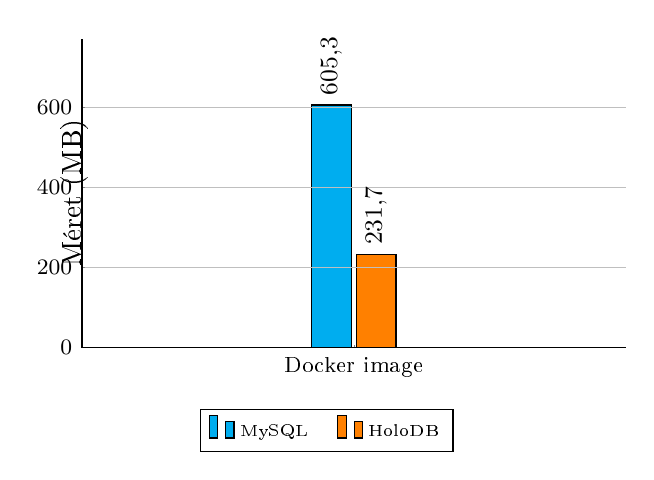
\begin{tikzpicture}
            \begin{axis}[
                    symbolic x coords={Docker image},
                    ybar,
                    axis on top,
                    width={0.7\textwidth},
                    height=5.5cm,
                    bar width=0.5cm,
                    ymajorgrids,
                    tick align=inside,
                    enlarge y limits={value=.1,upper},
                    enlarge x limits=0.15,
                    ymin=0,
                    ymax=700,
                    /pgf/number format/.cd,
                    use comma,
                    1000 sep={~},
                    point meta=rawy,
                    every node near coord/.append style={
                        anchor=west,
                        rotate=90,
                        font=\small
                    },
                    axis x line*=bottom,
                    axis y line*=left,
                    tickwidth=1pt,
                    legend style={
                        at={(0.45,-0.2)},
                        anchor=north,
                        legend columns=-1,
                        /tikz/every even column/.append style={column sep=0.3cm}
                    },
                    ylabel={Méret (MB)},
                    y label style={at={(0.03,0.5)}},
                    xtick=data,
                    nodes near coords={
                        \pgfmathprintnumber{\pgfplotspointmeta}
                    },
                    nodes near coords style={
                        /pgf/number format/.cd,
                        /pgf/number format/fixed,
                        precision=3
                    }
                ]
                \addplot[fill=cyan] % MySQL
                    coordinates { (Docker image,605.3) };
                \addplot[fill=orange] % HoloDB
                    coordinates { (Docker image,231.7) };
                \legend{MySQL,HoloDB}
            \end{axis}
        \end{tikzpicture}
    \end{minipage}%
    \begin{minipage}[b]{0.25\textwidth}
        \centering
        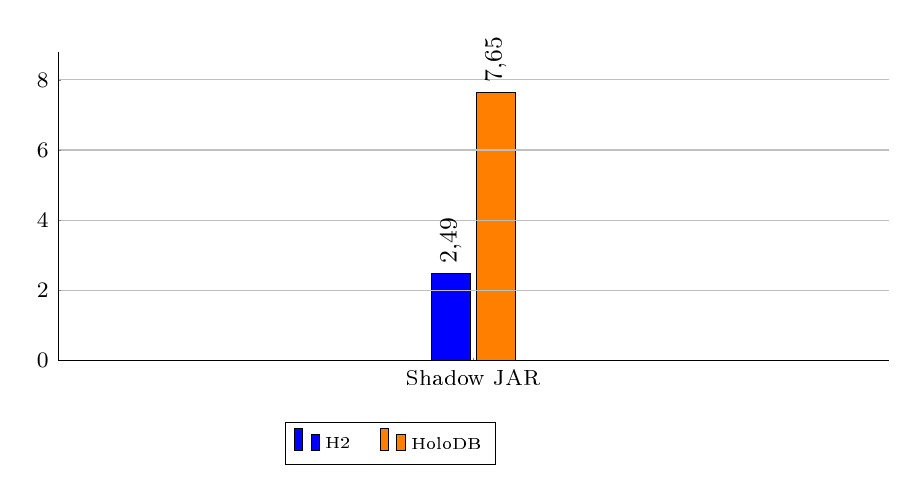
\begin{tikzpicture}
            \begin{axis}[
                    symbolic x coords={Shadow JAR},
                    ybar,
                    axis on top,
                    width={\textwidth},
                    height=5.5cm,
                    bar width=0.5cm,
                    ymajorgrids,
                    tick align=inside,
                    enlarge y limits={value=.1,upper},
                    enlarge x limits=0.15,
                    ymin=0,
                    ymax=8,
                    /pgf/number format/.cd,
                    use comma,
                    1000 sep={~},
                    point meta=rawy,
                    every node near coord/.append style={
                        anchor=west,
                        rotate=90,
                        font=\small
                    },
                    axis x line*=bottom,
                    axis y line*=left,
                    tickwidth=1pt,
                    legend style={
                        at={(0.4,-0.2)},
                        anchor=north,
                        legend columns=-1,
                        /tikz/every even column/.append style={column sep=0.3cm}
                    },
                    xtick=data,
                    nodes near coords={
                        \pgfmathprintnumber{\pgfplotspointmeta}
                    },
                    nodes near coords style={
                        /pgf/number format/.cd,
                        /pgf/number format/fixed,
                        precision=3
                    }
                ]
                \addplot[fill=blue] % H2
                    coordinates { (Shadow JAR,2.49) };
                \addplot[fill=orange] % HoloDB
                    coordinates { (Shadow JAR,7.65) };
                \legend{H2,HoloDB}
            \end{axis}
        \end{tikzpicture}
    \end{minipage}%
    \begin{minipage}[b]{0.3\textwidth}
        \centering
        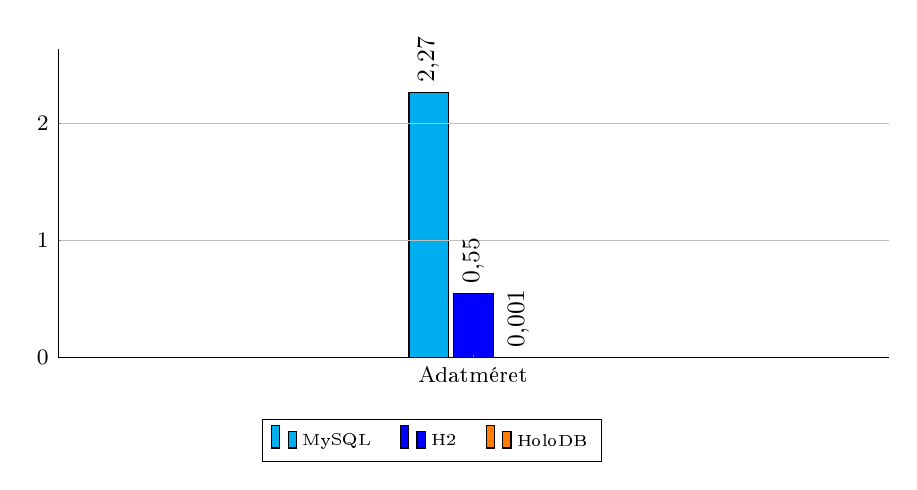
\begin{tikzpicture}
            \begin{axis}[
                    symbolic x coords={Adatméret},
                    ybar,
                    axis on top,
                    width={\textwidth},
                    height=5.5cm,
                    bar width=0.5cm,
                    ymajorgrids,
                    tick align=inside,
                    enlarge y limits={value=.1,upper},
                    enlarge x limits=0.15,
                    ymin=0,
                    ymax=2.4,
                    /pgf/number format/.cd,
                    use comma,
                    1000 sep={~},
                    point meta=rawy,
                    every node near coord/.append style={
                        anchor=west,
                        rotate=90,
                        font=\small
                    },
                    axis x line*=bottom,
                    axis y line*=left,
                    tickwidth=1pt,
                    legend style={
                        at={(0.45,-0.2)},
                        anchor=north,
                        legend columns=-1,
                        /tikz/every even column/.append style={column sep=0.3cm}
                    },
                    xtick=data,
                    nodes near coords={
                        \pgfmathprintnumber{\pgfplotspointmeta}
                    },
                    nodes near coords style={
                        /pgf/number format/.cd,
                        /pgf/number format/fixed,
                        precision=3
                    }
                ]
                \addplot[fill=cyan] % MySQL
                    coordinates { (Adatméret,2.27) };
                \addplot[fill=blue] % H2
                    coordinates { (Adatméret,0.55) };
                \addplot[fill=orange] % HoloDB
                    coordinates { (Adatméret,0.001) };
                \legend{MySQL,H2,HoloDB}
            \end{axis}
        \end{tikzpicture}
    \end{minipage}
\end{frame}

\begin{frame}
    \slidetitle{\sectionshorttitle}{Integrált teszt futási ideje (Micronaut$,$ REST)}
    
    \centering
    
    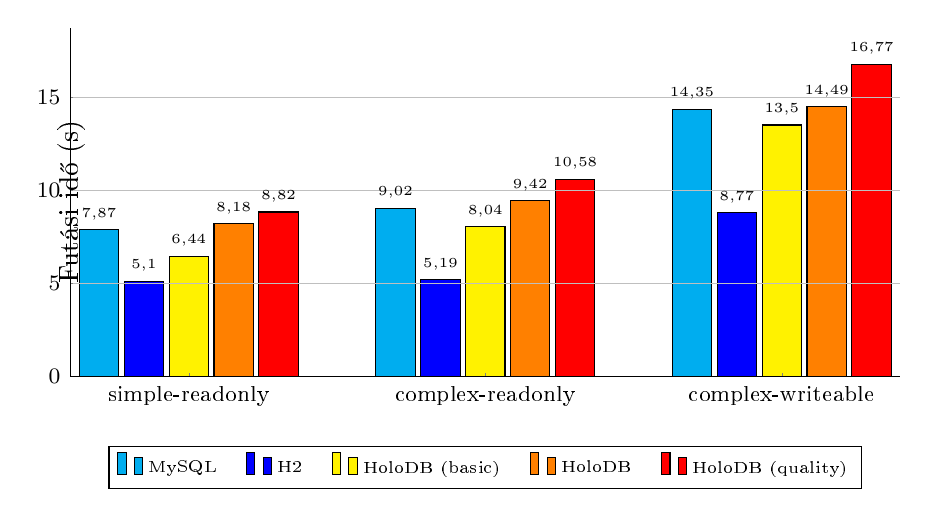
\begin{tikzpicture}[font=\tiny]
        \begin{axis}[
                symbolic x coords={simple-readonly,complex-readonly,complex-writeable},
                ybar,
                axis on top,
                width={\textwidth},
                height=6cm,
                bar width=0.5cm,
                ymajorgrids,
                tick align=inside,
                enlarge y limits={value=.1,upper},
                enlarge x limits=0.2,
                ymin=0,
                ymax=17,
                /pgf/number format/.cd,
                use comma,
                1000 sep={~},
                axis x line*=bottom,
                axis y line*=left,
                tickwidth=1pt,
                legend style={
                    at={(0.5,-0.2)},
                    anchor=north,
                    legend columns=-1,
                    font = {\fontsize{6 pt}{10 pt}\selectfont},
                    /tikz/every even column/.append style={column sep=0.3cm}
                },
                ylabel={Futási idő (s)},
                y label style={at={(0.03,0.5)}},
                xtick=data,
                nodes near coords={
                    \pgfmathprintnumber{\pgfplotspointmeta}
                }
            ]
            \addplot[fill=cyan] % MySQL
                coordinates {
                    (simple-readonly,7.870093628)
                    (complex-readonly,9.0179515675)
                    (complex-writeable,14.3489598653)
                };
            \addplot[fill=blue] % H2
                coordinates {
                    (simple-readonly,5.103988787)
                    (complex-readonly,5.1902669386)
                    (complex-writeable,8.7714582641)
                };
            \addplot[fill=yellow] % HoloDB (basic)
                coordinates {
                    (simple-readonly,6.441775179)
                    (complex-readonly,8.0399578991)
                    (complex-writeable,13.4957423082)
                };
            \addplot[fill=orange] % HoloDB
                coordinates {
                    (simple-readonly,8.182373242)
                    (complex-readonly,9.4207860077)
                    (complex-writeable,14.4941282014)
                };
                
            \addplot[fill=red] % HoloDB (quality)
                coordinates {
                    (simple-readonly,8.819935654)
                    (complex-readonly,10.5782986771)
                    (complex-writeable,16.7720866313)
                };
            \legend{MySQL,H2,HoloDB (basic),HoloDB,HoloDB (quality)}
        \end{axis}
    \end{tikzpicture}
\end{frame}

\begin{frame}
    \slidetitle{\sectionshorttitle}{SQL-futásidők átlagának összehasonlítása (log.)}
    
    \centering
    
    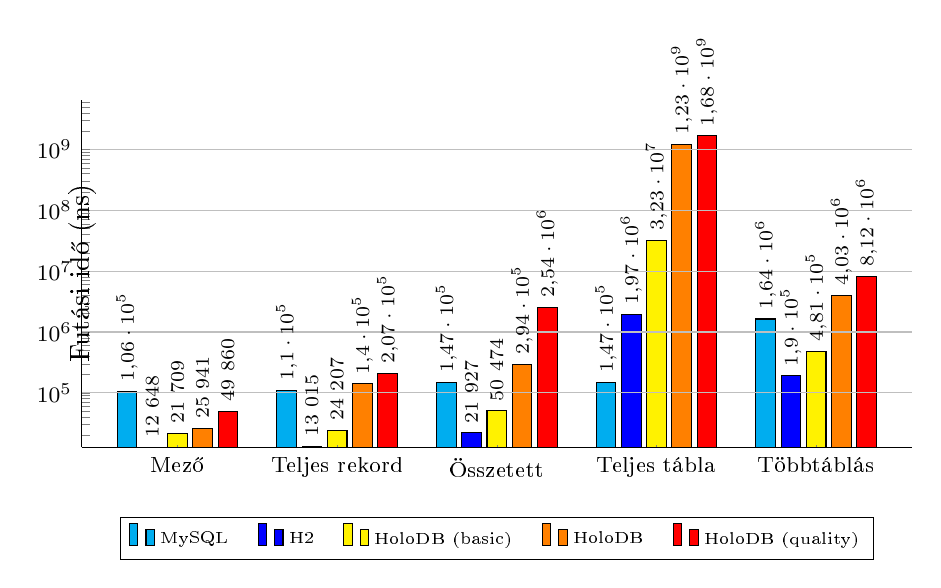
\begin{tikzpicture}[font=\scriptsize]
        \begin{axis}[
                title style={
                    at={(-0.1,1.15)},
                    anchor=north west
                },
                symbolic x coords={Mező,Teljes rekord,Összetett,Teljes tábla,Többtáblás},
                ybar,
                axis on top,
                width={\textwidth},
                height=6cm,
                bar width=0.25cm,
                ymajorgrids,
                tick align=inside,
                enlarge y limits={value=.1,upper},
                enlarge x limits=0.15,
                ymin=0,
                ymax=2000000000,
                ymode=log,
                point meta=rawy,
                /pgf/number format/.cd,
                use comma,
                1000 sep={~},
                every node near coord/.append style={
                    anchor=west,
                    rotate=90
                },
                axis x line*=bottom,
                axis y line*=left,
                tickwidth=1pt,
                legend style={
                    at={(0.5,-0.2)},
                    anchor=north,
                    legend columns=-1,
                    font = {\fontsize{6 pt}{10 pt}\selectfont},
                    /tikz/every even column/.append style={column sep=0.3cm}
                },
                ylabel={Futási idő (ns)},
                y label style={at={(0.03,0.5)}},
                xtick=data,
                nodes near coords={
                    \pgfmathprintnumber{\pgfplotspointmeta}
                }
            ]
            \addplot[fill=cyan] % MySQL
                coordinates {
                    (Mező,106276)
                    (Teljes rekord,109819) 
                    (Összetett,146710)
                    (Teljes tábla,146710)
                    (Többtáblás,1637889)
                };
            \addplot[fill=blue] % H2
                coordinates {
                    (Mező,12648)
                    (Teljes rekord,13015) 
                    (Összetett,21927)
                    (Teljes tábla,1971234)
                    (Többtáblás,189958)
                };
            \addplot[fill=yellow] % HoloDB (basic)
                coordinates {
                    (Mező,21709)
                    (Teljes rekord,24207) 
                    (Összetett,50474)
                    (Teljes tábla,32271101)
                    (Többtáblás,481306)
                };
            \addplot[fill=orange] % HoloDB
                coordinates {
                    (Mező,25941)
                    (Teljes rekord,140232) 
                    (Összetett,293885)
                    (Teljes tábla,1228183178)
                    (Többtáblás,4030303)
                };
            \addplot[fill=red] % HoloDB (quality)
                coordinates {
                    (Mező,49860)
                    (Teljes rekord,207383) 
                    (Összetett,2543441)
                    (Teljes tábla,1676796378)
                    (Többtáblás,8121736)
                };
            \legend{MySQL,H2,HoloDB (basic),HoloDB,HoloDB (quality)}
        \end{axis}
    \end{tikzpicture}
\end{frame}

\section{Összegzés}
\def\sectionshorttitle{\arabic{section}. Összegzés}

\begin{frame}
    \slidetitle{\sectionshorttitle}{Elvárások teljesítése}
    
    \begin{itemize}
        \setlength\itemsep{0.5em}
        \item[\greencheck] {\color{red}relációs adatmodell}re épül
        \item[\greencheck] {\color{red}deklaratív}, finomhangolható, könnyen bővíthető
        \item[\greencheck] {\color{red}nincs preparálás}i folyamat, szinte azonnal elindul
        \item[\greencheck] óriás adatmennyiséget is képes szimulálni, szinte {\color{red}tárhelyigény nélkül}
        \item[\greencheck] az adatokat csak elérésükkor, on-the-fly számítja
        \item[\greencheck] indexelt, a runtime teljesítmény elfogadható
        \item[\greencheck] determinisztikus, {\color{red}koherens}, skálázható
        \item[\greencheck] opcionálisan írható
    \end{itemize}
\end{frame}

\begin{frame}
    \slidetitle{\sectionshorttitle}{További lehetőségek}
    
    \begin{itemize}
        \setlength\itemsep{1em}
        \item könnyen verziókezelhető
        \item könnyen replikálható (csak-olvasható adatbázis esetén)
        \item JPA-entitásokból is indítható (nem szükséges a YAML-fájl)
        \item füsttesztekhez is használható
        \item akár serverless szolgáltatásként is működtethető
        \item az írási réteg meglévő adatbázis fölé is elhelyezhető
        \item a konfiguráció újraindítás nélkül is újratölthető
    \end{itemize}
\end{frame}

\begin{frame}
    \slidetitle{\sectionshorttitle}{A közeljövő fő tervei}

    A meglévő funkciók továbbfejlesztésén, optimalizálásán túl:
    
    \vspace{1em}
    
    \begin{itemize}
        \setlength\itemsep{1em}
        \item további értékkészlet-típusok
        \item könnyen konfigurálható megkötések
        \item DBeaver-integráció
        \item általános keretrendszer letapogatáshoz és materializáláshoz
        \item HoloDB mint felhőszolgáltatás
        \item igényfelmérés, alkalmazás valós projekteken
    \end{itemize}
\end{frame}
        
\begin{frame}
    \vspace{1em}
    
    \centering
    
    { \Huge Köszönöm a figyelmet! }
    
    \vspace{3em}
    
    \hspace*{\fill}%
    \begin{minipage}[c]{0.75\textwidth}
        \begin{flushleft}
            \normalsize
            
            ~~~
            {\color{beamer@blendedblue}Linkek:}
            
            \vspace{0.5em}
            
            \footnotesize
            
            \begin{itemize}
                \item HoloDB projekt: \par
                    \url{https://github.com/miniconnect/holodb}
                \item Használati példák: \par
                    \scriptsize{\url{https://github.com/miniconnect/general-docs/tree/main/examples}}
                \item Jelen TDK-pályamunka forrásrepója: \par
                    \url{https://github.com/davidsusu/holodb-tdk}
            \end{itemize}
            
            \vspace{1.5em}
            
            \normalsize
            
            ~~~
            { \color{beamer@blendedblue} E-mail: }
            \href{mailto:horvathdown@student.elte.hu}{horvathdown@student.elte.hu}
        \end{flushleft}
    \end{minipage}%
    \hspace*{\fill}%
    \begin{minipage}[c]{0.24\textwidth}
        \scalebox{1.5}{\qrcode{https://github.com/miniconnect/holodb}}
    \end{minipage}%
    \hspace*{\fill}%
\end{frame}

\appendix
\begingroup
\setbeamertemplate{footline}{}

\section{Bírálói kérdések}
\def\sectionshorttitle{Kérdések}

\begin{frame}[c,noframenumbering]
    ~~~
    
    \brqr
\end{frame}

\begin{frame}[c,noframenumbering]
    \centering
    
    \Huge Bírálói kérdések
    
    \brqr
\end{frame}

\begin{frame}[t,noframenumbering]
    \slidetitle{\sectionshorttitle}{1. Több SQL dialektus}
    
    \textbf{%
    Tudna-e a rendszer támogatni különböző query nyelveket
    egy absztrakciós rétegen keresztül,
    hogy integrálni lehessen olyan rendszerekkel,
    amelyek kötve vannak egy bizonyos SQL típushoz?
    }
    
    \vspace{0.7cm}
    
    \begin{itemize}
        \setlength\itemsep{1em}
        \item \textbf{igen}
        \begin{itemize}
            \item a \texttt{QueryExecutor} implementációja cserélhető, jelenleg kétféle lehet:
            \begin{itemize}
                \item \texttt{default} (limitált SQL, gyors)
                \item Apache Calcite (kb. 40-féle dialektust támogat)
            \end{itemize}
            \item kezdetleges támogatás további lekérdezési módokhoz is elérhető:
            \begin{itemize}
                \item REST API
                \item GraphQL (GraphQL-Java)
                \item SPARQL (Quetzal)
            \end{itemize}
        \end{itemize}
    \end{itemize}
    
    \brqr
\end{frame}

\begin{frame}[t,noframenumbering,fragile]
    \slidetitle{\sectionshorttitle}{2. ORM-integráció}
    
    \textbf{%
    Lehetne-e integrációt nyújtani meglévő ORM keretrendszerekhez
    (pl. Hibernate)?
    Mennyire látja ezt megvalósíthatónak?
    }
    
    \vspace{0.3cm}
    
    \begin{itemize}
        \setlength\itemsep{1em}
        \item \textbf{támogatott}: konfiguráció helyett JPA entitások (opcionális kiegészítő annotációkkal):
    \end{itemize}
    
    \hspace*{0.05\textwidth}
    \begin{minipage}{0.72\textwidth}
        \begin{minted}[
            fontsize=\tiny,
            framesep=4pt,
            frame=single,
            framerule=1.5pt,
            rulecolor=\color{gray!30}
        ]{java}
@Entity
@Table(name = "posts")
@HoloTable(size = 500)
public class Post {
    @Id
    @GeneratedValue(strategy = GenerationType.IDENTITY)
    private Long id;
    
    @Column
    @HoloColumn(valuesBundle = "lorem")
    private String title;

    @Column(name = "tag")
    @ElementCollection
    @CollectionTable(name = "post_tags", joinColumns = { @JoinColumn(name = "post_id") })
    @HoloTable(size = 20)
    @HoloColumn(values = { "tag1", "tag2", "tag3" })
    @HoloVirtualColumn(name = "color", valuesBundle = "colors")
    private Set<String> tags;

    // ...
        \end{minted}
    \end{minipage}
    
    \brqr
\end{frame}

\begin{frame}[t,noframenumbering]
    \slidetitle{\sectionshorttitle}{3. Komplex megkötések}
    
    \textbf{%
    Tudna-e támogatni a megoldás egy tábla oszlopai közötti
    vagy akár különböző táblák közötti
    strukturális és komplex kényszereket?
    }
    
    \vspace{0.7cm}
    
    \begin{itemize}
        \setlength\itemsep{1em}
        \item jelenleg csak \textbf{részlegesen}
        \begin{itemize}
            \item konfigurációból jelenleg csak részhalmaz megkötések (pl. idegen kulcs) adhatók meg
            \item többoszlopos \texttt{Source} egyedileg hozzáadható
            \item más értékektől függő, nem indexelt \texttt{Source} egyedileg hozzáadható
        \end{itemize}
        \item minél több megkötés támogatása prioritás, már tervezés alatt:
        \begin{itemize}
            \item "kombinatorikus" virtuális index
            \item kényszerek könnyű konfigurálhatósága
        \end{itemize}
    \end{itemize}
    
    \brqr
\end{frame}

\endgroup

\end{document}
